Эксперимент 1.

На рисунке 2 представлены графики изменения $a(x)$ и $b(x)$, в зависимости от $x$, на рисунке 3 ряд распределения вероятностей количества заявок на орбите для следующих параметров системы $N=2$, $r_{0}=0,5, r_{1}=0,2, r_{2}=0,3, \lambda=0,8, \mu_{1}=1,2, \mu_{2}=0,6 , q=0,8, \sigma=0.2.$

\begin{figure}[H]
	\centering
	\begin{minipage}[h]{0.49\linewidth}
		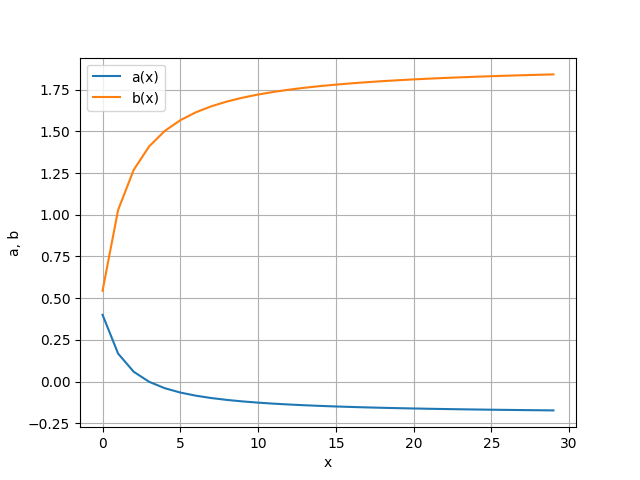
\includegraphics[width=0.8\linewidth]{ab2} 	
		\caption{Коэффициенты переноса $a(x)$ и диффузии $b(x)$}
		\label{ris:experimoriginal}
	\end{minipage}
	\hfill
	\begin{minipage}[h]{0.49\linewidth}
		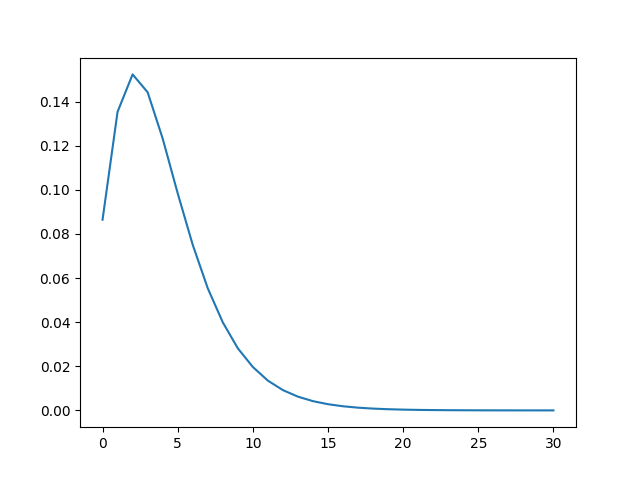
\includegraphics[width=0.8\linewidth]{P2} 
		\caption{Ряд распределения вероятностей числа заявок на орбите}
		\label{ris:experimcoded}
	\end{minipage}
\end{figure}
\noindent Эксперимент 2.

На рисунке 4 представлены графики изменения $a(x)$ и $b(x)$, в зависимости от $x$, на рисунке 5 ряд распределения вероятностей количества заявок на орбите для следующих параметров системы $N=10$, $r_{0}=0,5, r_{1}=0,2, r_{2}=0,3, \lambda=0,8, \mu_{1}=1,2, \mu_{2}=0,6 , q=0,8, \sigma=0.1.$
\begin{figure}[H]
	\centering
	\begin{minipage}[h]{0.49\linewidth}
		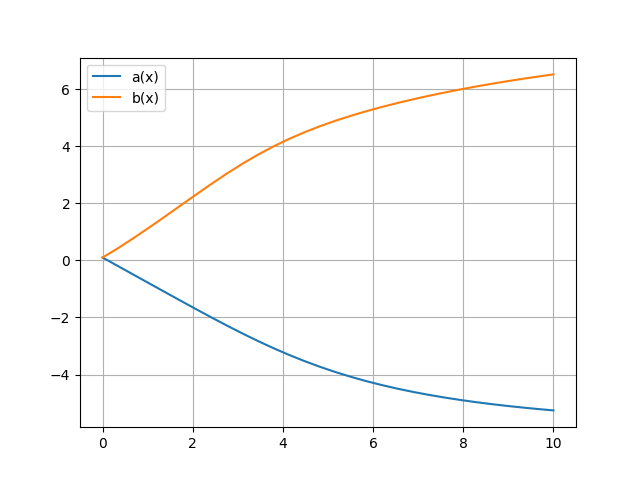
\includegraphics[width=0.8\linewidth]{ab10} 	
		\caption{Коэффициенты переноса $a(x)$ и диффузии $b(x)$}
		\label{ris:experimoriginal}
	\end{minipage}
	\hfill
	\begin{minipage}[h]{0.49\linewidth}
		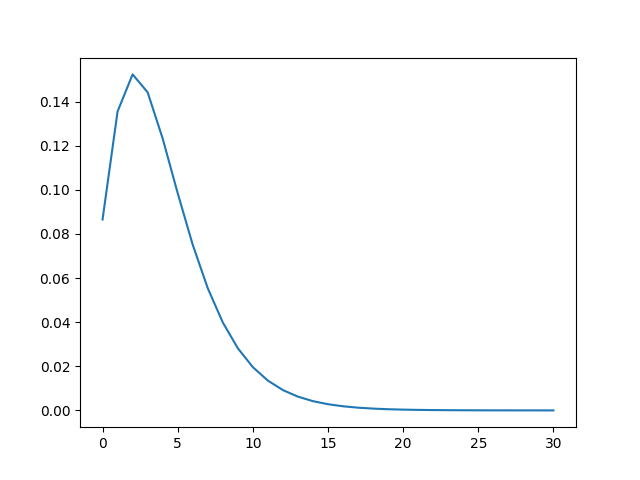
\includegraphics[width=0.8\linewidth]{P10} 
		\caption{Ряд распределения вероятностей числа заявок на орбите}
		\label{ris:experimcoded}
	\end{minipage}
\end{figure}

Численные результаты были получены с помощью библиотек NymPy [20] (для $a(x)$ и $b(x)$) языка программирования Python, реализация выложена в открытый доступ [14].
Данные графики были построены с помощью библиотеки Matplotlib [17] языка Python.

Сравним полученные результаты с имитационной моделью [16]. Для этого обозначим ряд распределения вероятностей числа заявок на орбите, полученный в результате [16], -- $P^{(2)}(i)$ и представим на рисунке 6 $P(i)$  и $P^{(2)}(i)$ для следующих параметров системы $N=64$, $r_{0}=0,5, r_{1}=0,2, r_{2}=0,3, \lambda=40,96, \mu_{1}=1,2, \mu_{2}=0,6 , q=0,8, \sigma=0.2.$
\begin{figure}[H]
	\centering
	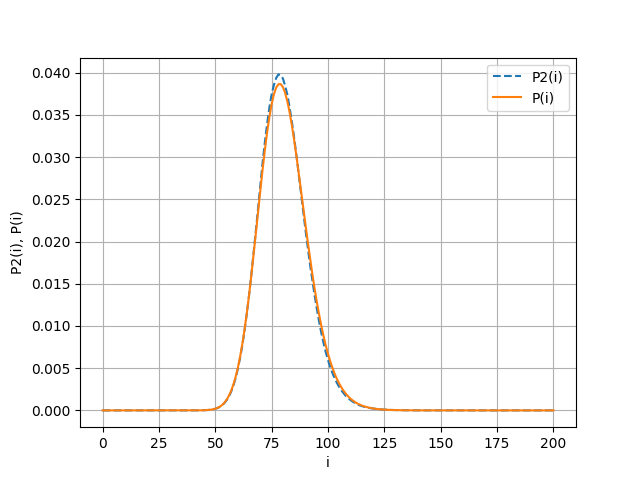
\includegraphics[width=0.6\linewidth]{pic64_0_2.png} 
	\caption{Ряд распределения вероятностей числа заявок на орбите, полученный численно $P(i)$ и с помощью имитационной модели $P^{(2)}(i)$}
	\label{ris:experimcoded}
\end{figure}
Визуально два ряда распределения вероятности выглядят очень близкими.
Для сравнения двух распределений вероятностей численно будем использовать расстояние Колмогорова
\begin{equation*}
	\Delta=\max_{0 \leq  n \leq  \infty}\bigg|\sum_{i=0}^{n}(P(i)-P^{(2)}(i))\bigg|.
\end{equation*}

Приведем полученные результаты в таблице 1 для изменяющегося числа приборов $N$ и $\sigma$.

\captionsetup[table]{justification=raggedright}
\begin{table}[h]
	\caption{Расстояние Колмогорова}
	 \centering 
	\begin{tabular}{ | c | c | c | c | c | }
		\hline
		$\Delta$ & $\sigma=5$ & $\sigma=1$ & $\sigma=0,2$  & $\sigma=0,04$ \\ \hline
		$N=2$ & 0,02124 & 0,02185 & 0,00179 & 0,00060 \\ \hline
		$N=4$ & 0,03852 & 0,02108 & 0,00206 & 0,00030 \\ \hline
		$N=16$ & 0,07338 & 0,01649 & 0,00266 & 0,00056 \\ \hline
		$N=64$ & 0,03329 & 0,00582 & 0,00176 & 0,00032 \\ 
		\hline
	\end{tabular}
\end{table}
